\chapter{ĐIỀU KHIỂN ĐỘNG CƠ DC}
\section{Giới thiệu chung}
\subsection{Yêu cầu}Điều khiển chiều quay và tốc độ động cơ DC.
\subsection{Động cơ DC}
Để động cơ hoạt động được, ta cấp điện áp vào động cơ, xuất hiện dòng điện chạy các cuộn dây trong động cơ, làm động cơ quay theo một chiều xác định, để đổi chiều quay ta đổi chiều điện áp. Khi điều khiển động cơ: không được cấp điện áp và dòng điện quá giá trị định mức ghi trên động cơ (cấp thấp hơn động cơ vẫn hoạt động được).
\section{Các bài toán điều khiển động cơ}
\subsection{Điều khiển chiều quay của động cơ}
Để điều khiển chiều quay của động cơ, người ta sử dụng mạch cầu H để làm điều này.

\begin{figure}[!h]
\begin{center}
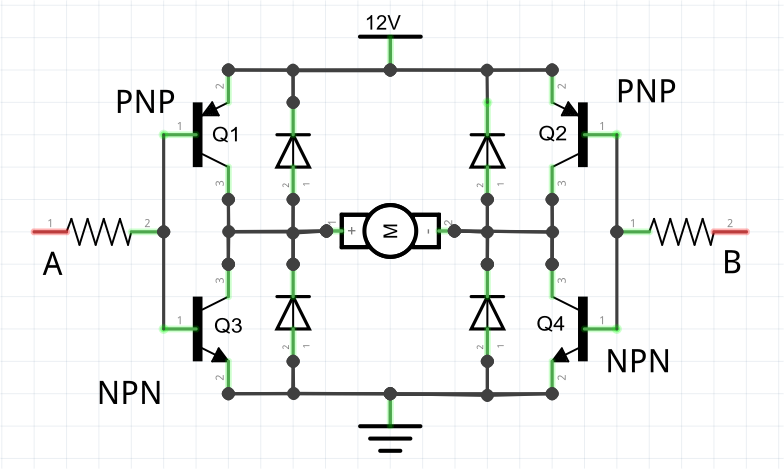
\includegraphics[scale=0.3]{bai-8/image/mach-cau-H}
\end{center}
\caption{Mạch cầu H điều khiển chiều quay của động cơ}
\end{figure}
\newpage
Chọn IC L293D để thực hiện chức năng của mạch cầu H điều khiển chiều quay của động cơ. Cụ thể như sau:
\begin{figure}[!h]
\begin{center}
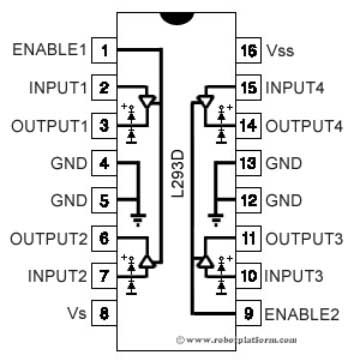
\includegraphics[scale=0.35]{bai-8/image/L293D}
\end{center}
\caption{Sơ đồ chân IC L293D}
\end{figure}
\begin{itemize}
\item Số chân của IC: 16 chân (6 chân điều khiển tín hiệu; 4 chân điều khiển động cơ; 2 chân cấp nguồn; 4 chân đất), IC điều khiển được 2 động cơ.
\item Các chân điều khiển: \verb|ENABLE1|, \verb|INPUT1|, \verb|INPUT2| (động cơ 1) và \verb|ENABLE2|, \verb|INPUT3|, \verb|INPUT4| (động cơ 2). Cụ thể chiều quay được xác định như sau:
\begin{itemize}
\item[$\ast$] Ta xác định cách điều khiển cho động cơ thứ nhất.
\item Chiều ngược chiều kim đồng hồ: \verb|ENABLE1 = 1|, \verb|INPUT1 = 1|, \verb|INPUT2 = 0|.
\item Chiều cùng chiều kim đồng hồ: \verb|ENABLE1 = 1|, \verb|INPUT1 = 0|, \verb|INPUT2 = 1|.
\item Dừng động cơ khi \verb|ENABLE1 = 0| (bất kể \verb|INPUT1| và \verb|INPUT2| ở mức cao hay mức thấp).
\item[$\ast$] Động cơ thứ 2 cũng thực hiện tương tự như vậy: ta dùng các chân \verb|ENABLE2|, \verb|INPUT3|, \verb|INPUT4|.
\end{itemize}
\item Cấp nguồn: chân \verb|VSS| lấy nguồn của vi điều khiển, chân \verb|Vs| lấy nguồn ngoài cấp cho động cơ (không nên dùng chung nguồn với vi điều khiển).
\item Chân nối động cơ: \verb|OUTPUT1|, \verb|OUTPUT2| cho động cơ 1; \verb|OUTPUT3|, \verb|OUTPUT4| cho động cơ 2.
\end{itemize}
\subsection{Điều khiển tốc độ quay của động cơ}
Ta sử dụng phương pháp điều chế độ rộng xung -- \verb|PWM| để điểu khiển tốc độ động cơ. Ví dụ như trong các giản đồ xung \textit{hình \ref{pwm}}:
\begin{figure}[!h]
\begin{center}
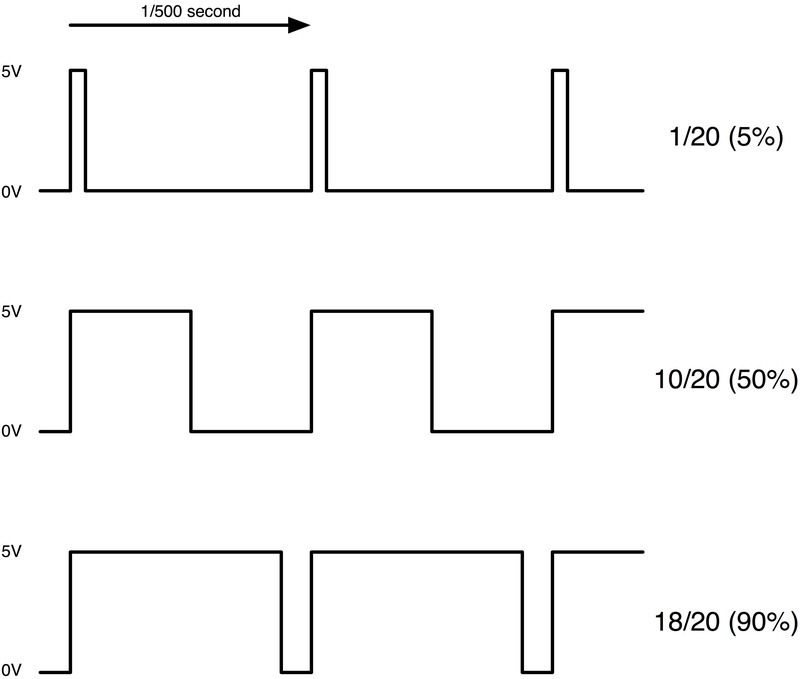
\includegraphics[width=.3\linewidth]{bai-8/image/pwm-1}
\end{center}
\caption{Phương pháp điều chế độ rộng xung} \label{pwm}
\end{figure}

Khối \verb|PWM| trên PIC 16F887 có 2 mạch so sánh: \verb|8 bit| (so sánh với giá trị đếm của \verb|timer2|) và \verb|10 bit|.\\

Ta thực hiện điều chế độ rộng xung bằng phần cứng (dùng chân \verb|CCP1| hoặc \verb|CCP2|). Tiến hành tính toán và thiết lặp các giá trị sau:
\begin{itemize}
\item Xác định tần số điều xung \verb|PWM| qua khai báo sau:

\verb|setup_timer_2(mode, period, postscale);|

suy ra: $\displaystyle f = \frac{f_{osc}}{4 \times mode \times \left({period+1}\right)}$ với:
\begin{itemize}
\item \verb|mode|: \verb|T2_DIV_BY_1|, \verb|T2_DIV_BY_4|, \verb|T2_DIV_BY_16|.
\item \verb|period|: $0-255$.
\item \verb|postscale|: $1$.
\end{itemize}
\item Kích hoạt chế độ \verb|PWM|: \verb|setup_ccp1(cpp_pwm)| hoặc \verb|setup_ccp2(cpp_pwm)|.
\item Xác định hệ số chu kỳ xung thông qua khai báo:


\verb|set_pwm1_duty(value)| hoặc \verb|set_pwm2_duty(value)|
\begin{itemize}
\item Nếu \verb|value| là số nguyên 8 bit: $\displaystyle duty cycle = \frac{value}{period + 1}$.
\item Nếu \verb|value| là số nguyên 16 bit: $\displaystyle duty cycle = \frac{value \times 1023}{4 \times \left({period + 1}\right)}$.
\end{itemize}
\item[$\ast$] Nếu ứng dụng không cần điều chế xung mịn thì ta có thể dùng \textit{8 bit}.
\end{itemize}
\section{Bài tập}
\subsection{Bài tập 8.1}
\paragraph{Yêu cầu}Viết chương trình điều khiển chiều quay động cơ bằng nút nhấn nối với ngắt ngoài của vi điều khiển PIC 16F887.
\paragraph{Hướng giải quyết}
\begin{itemize}
\item Ta sử dụng ngắt ngoài \verb|#INT_EXT| (ngắt trên chân B0) để điều khiển chiều quay của động cơ thông qua số lần nhấn nút \verb|count|:
\item Khi chưa nhấn nút nhấn (\verb|count = 0|): động cơ chưa quay.
\item Khi nhấn nút lần đầu tiên (\verb|count%2 = 1|): động cơ quay theo chiều thuận: \verb|ENABLE1 = 1|, \verb|INPUT1 = 1|, \verb|INPUT2 = 0|.
\item Khi nhấn nút lần thứ 2 (\verb|count%2 = 0|): động cơ quay theo chiều nghịch: \verb|ENABLE1 = 1|, \verb|INPUT1 = 0|, \verb|INPUT2 = 1|.
\item Lặp lại quá trình trên.
\item \textit{Lưu ý}: tùy vào phần cứng của chúng ta có bị nhiễu hay không mà ta có thể khai báo giá trị ban đầu của biến \verb|count| là: \verb|count = 0| hay \verb|count = -1|.
\end{itemize}
\newpage
\subsection*{Sơ đồ mạch}
\begin{figure}[!h]
\begin{center}
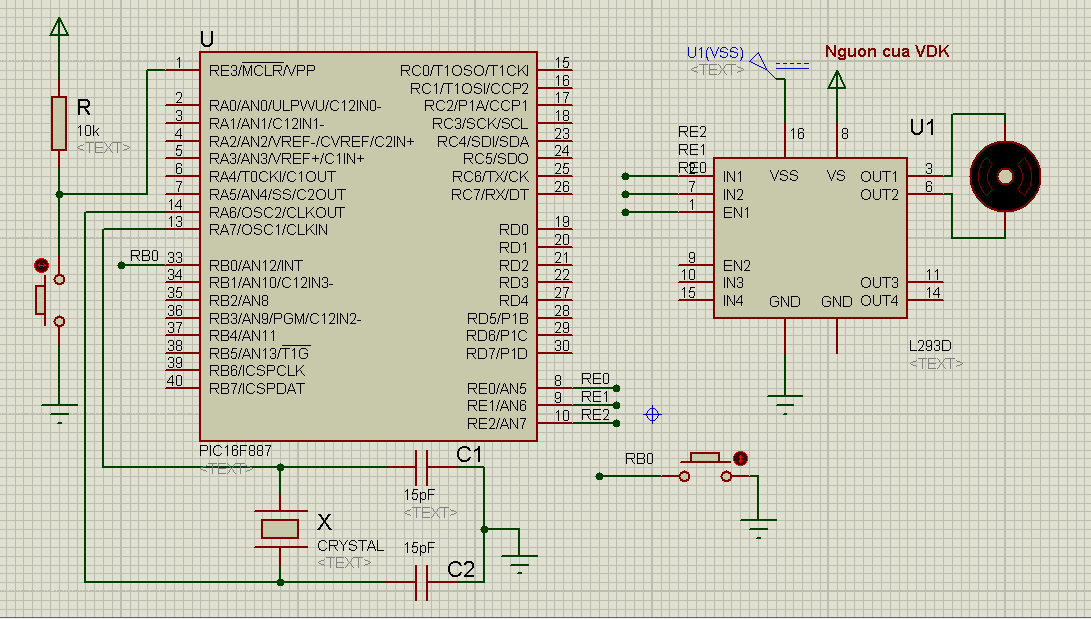
\includegraphics[scale=0.5]{bai-8/image/BAI-8-1}
\end{center}
\caption{Mạch đảo chiều động cơ với IC L293D}
\label{Fig:dao-chieu}
\end{figure}
\subsection*{Chương trình 23}
\lstinputlisting[language=C]{BAI-8-1.C}
\subsection{Bài tập 8.2}
\paragraph{Yêu cầu}Viết chương trình điều khiển tốc độ và chiều quay của động cơ.
\paragraph{Hướng giải quyết}
\begin{itemize}
\item Do đề bài không đưa ra yêu cầu cụ thể là điều khiển như thế nào, nên ta đặt ra yêu cầu cụ như sau:
\begin{itemize}
\item Khi chưa nhấn nút nhấn trạng thái 0: động cơ không quay.
\item Khi nhấn nút nhấn lần đầu tiên -- trạng thái 1: động cơ quay theo chiều của kim đồng hồ (quay thuận) và tốc độ tăng dần sau mỗi $1s$, đến khi ổn định tốc độ thì giảm dần tốc độ sau mỗi $1s$.
\item Nhấn nút nhấn lần thứ 2 -- trạng thái 2: động cơ quay ngược chiều của chiều kim đồng hồ (quay nghịch) và tốc độ tăng dần sau mỗi $1s$, đến khi ổn định tốc độ thì giảm dần tốc độ sau mỗi $1s$.
\end{itemize}
\item Ví dụ, ta cần điều chế một xung có tần số điều xung là $f = 10kHz$ thì ta cần chọn: $\displaystyle mode \times \left({period + 1}\right) = \frac{f_{osc}}{4 \times f} = \frac{20 \times 10^6}{4 \times 10 \times 10^3} = 500$, ta có bảng:
\begin{center}
\begin{tabular}{c|c}
\textit{mode} & \textit{period}\\ \hline
$1$ & $499$\\
$4$ & $124$\\
$16$ & $30.25$\\
\end{tabular}
\end{center}
Chọn cách khai báo sau: \verb|setup_timer_2(T2_DIV_BY_4,124,1);| sẽ tạo ra được một xung có tần số là $10kHz$.
\item Tăng hoặc giảm tốc độ, ta cần tăng hoặc giảm giá trị của tham số \verb|value| trong hàm \verb|set_pwm1_duty(value)|.

Ta giả sử \verb|set_pwm1_duty(dutycycle) = 100%|, thì xem \verb|value| có giá trị là bao nhiêu:
\begin{align*}
value & = \frac{1}{f} \times dutycycle \times \frac{f_{osc}}{mode} \\
& = \frac{1}{10kHz} \times 100\% \times \frac{20MHz}{4} \\
& = \frac{1}{10\times 10^3} \times 1 \times \frac{20 \times 10^6}{4} = 500
\end{align*}
\item Thực hiện vòng lặp \verb|for| tăng dần giá trị của \verb|value| nhưng phải luôn kiểm tra điều kiện $value \leq 500$.
\item Phần trên ta chỉ điều khiển được tốc độ, tiếp theo ta sẽ điều khiển chiều quay của động cơ: sử dụng IC L293D với chân \verb|ENABLE1| nối tắt lên nguồn, còn 2 chân \verb|INPUT1| và \verb|INPUT2| ta nối với 2 chân \verb|CCP1| và \verb|CCP2| để điều chế độ rộng xung cấp cho động cơ, việc đảo chiều tương tự như \textit{bài tập 8.1 trong chương trình 23}.
\item Cấu hình các chân điều khiển: \verb|PORTB = 0xFF| (chân \verb|INPUT|) và \verb|PORTC = 0x00| (chân \verb|OUTPUT|). Ta vẫn sử dụng ngắt ngoài ở B0 để dùng lại \textit{chương trình 23}.
\end{itemize}
%\subsection*{Sơ đồ mạch}
\paragraph{Sơ đồ mạch} giống sơ đồ \textit{bài tập 8.1} \textit{hình \ref{Fig:dao-chieu}} \textit{trang \pageref{Fig:dao-chieu}}.
\begin{comment}
\begin{figure}[!h]
\begin{center}
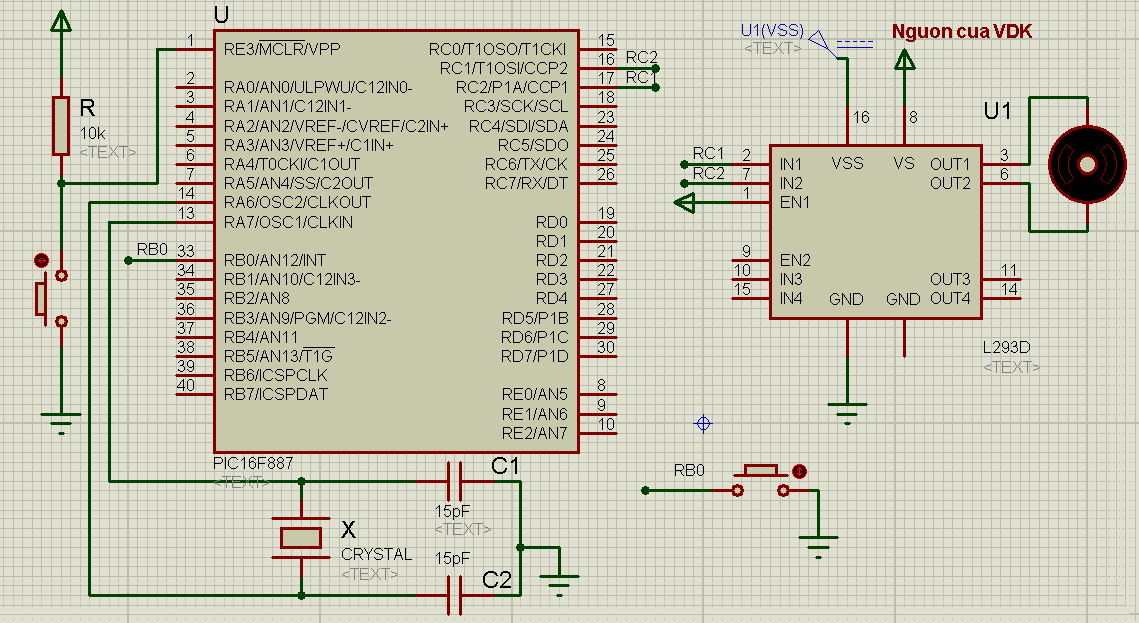
\includegraphics[scale=0.5]{bai-8/image/BAI-8-2}
\end{center}
\caption{Mạch đảo chiều động cơ và điều khiển tốc độ với IC L293D}
\end{figure}
\end{comment}
\subsection*{Chương trình 24}
\lstinputlisting[language=C]{BAI-8-2.C}
%\subsection{Bài tập 8.3}
%\paragraph{Yêu cầu}Viết chương trình đo tốc độ động cơ DC và hiển thị lên LCD 16x02.
%\subsection*{Chương trình 25}
%\subsection{Bài tập 8.4}
%\paragraph{Yêu cầu}Viết chương trình điều khiển tốc độ động cơ DC bằng PC qua cổng RS232.
%\paragraph{Hướng giải quyết}
%\begin{itemize}
%\item[$\ast$] Ta dự theo \textit{chương trình 24} của \textit{bài tập 8.2} với một số thay đổi phù hợp.
%\end{itemize}
%\subsection*{Chương trình 26}
\subsection{Điều khiển tốc độ động cơ với Transistor}
\paragraph{Sơ đồ mạch}{~\\}
\begin{figure}[!h]
\begin{center}
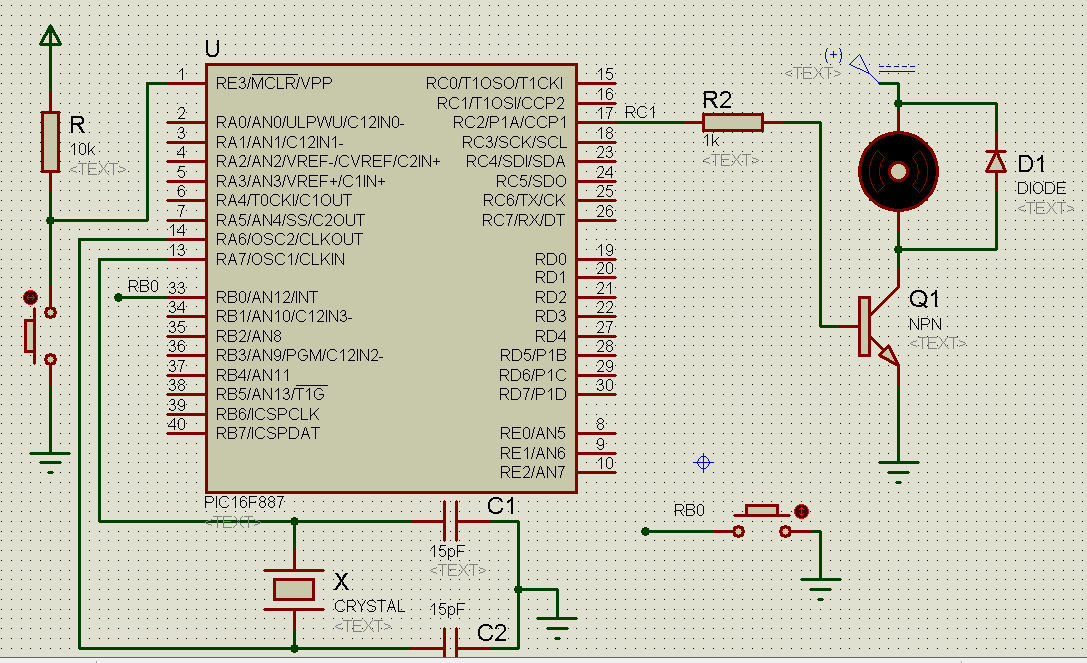
\includegraphics[scale=.5]{bai-8/image/BAI-8-2-2}
\end{center}
\caption{Điều khiển tốc độ động cơ với Transistor}
\end{figure}\\

Nội dung của chương trình: 
\subsection*{Chương trình 25}
\lstinputlisting[language=C]{BAI-8-2-1.C}